% Imporditud: tools/import_eksperimendid.py
% Allikas: Eesti füüsikaolümpiaadi eksperimendi ülesannete
%   kogu (Rael Kalda, 2023), ülesanne Ü179, lahendus L179.
\setAuthor{Jaan Kalda}
\setRound{lõppvoor}
\setYear{2021}
\setNumber{G E2}
\setDifficulty{5}
\setTopic{vedelike mehaanika}
\setVahendid{majapidamispaberi leht, anum veega, käärid, joonlaud}
\setPunktid{14}
\setAllikas{Eksperimendi kogu Ü179, lahendus lk 142}
\setLahendusseis{toores}

\prob{Majapidamispaber}
Hinnake majapidamispaberi kiudude vahelist keskmist vahekaugust. Kirjeldage võimalikult täpselt oma mõõtmisprotseduuri. Juuresolevalt mikroskoobi abil tehtud fotolt on näha, millised näevad välja majapidamispaberi kiud. Vee pindpinevustegur $\sigma$ = 0,072 N m$^{-1}$.

Pildi autoriõigused: Zephyris, CC BY-SA 3.0, via Wikimedia Commons.
\begin{center}
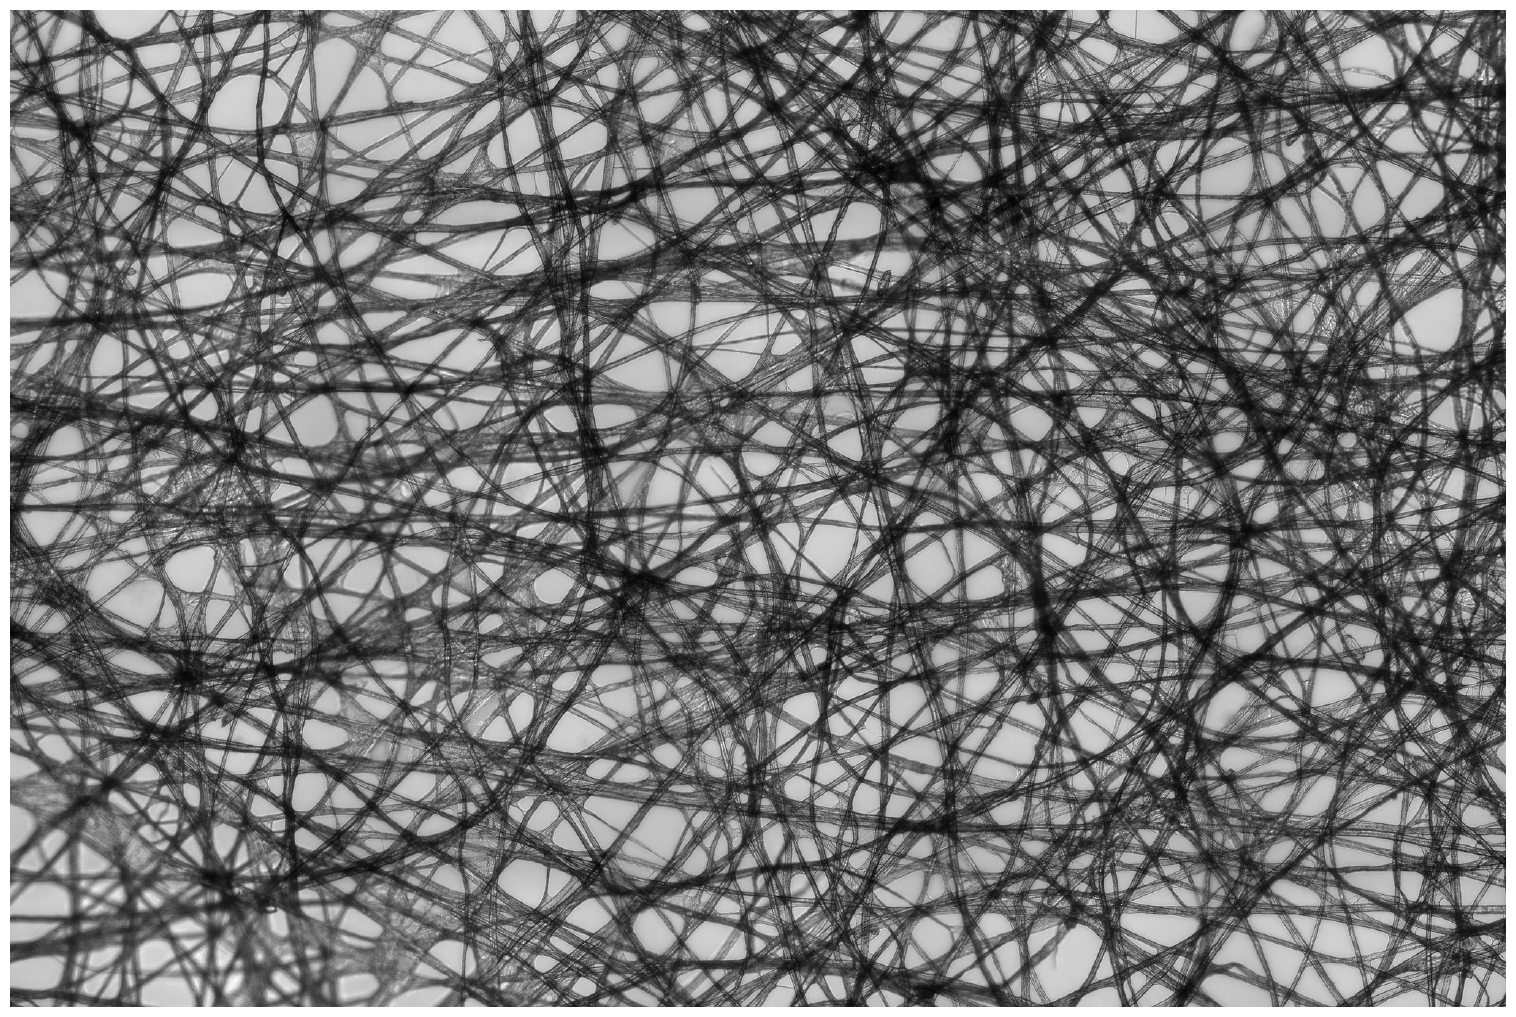
\includegraphics[width=0.75\linewidth]{2021-v3g-ge2-yl.png}
\\[2pt]{\footnotesize Pildi autoriõigused: Zephyris, CC BY-SA 3.0, via Wikimedia Commons.}
\end{center}
\textit{Vihje:} vedelikupinna kaks mõttelist poolt tõmbavad üksteist jõuga F = $\sigma$l, kus l on mõttelise eraldusjoone pikkus.

\hint

\solu
Lõikame paberist pika riba ja riputame otsapidi vette ning ootame seni, kuni vee mööda paberit ``üles ronimine'' peatub. See võtab üsna kaua, vähemalt paar minutit. Mõõdame märgunud osa kõrguse h mõõdetuna kõrgusena veepinnast, olgu see nt h = 75 mm. Pooride vahekauguse hindamiseks võime kasutada kapillaarrõhu valemit rõhu jaoks kõvera pinna all: paberi märgunud osa ülaservas vees on rõhk atmosfäärirõhust väiksem $\Delta$p = $\rho$gh võrra, kus $\rho$ = 1 g/cm$^3$, selle peab kompenseerima kapillaarrõhk, mis oleks silindrilise toru ja täieliku märgamise puhul 4$\sigma$/d. Suurusjärgulise hindamise puhul võime kasutada seda valemit asendades silindri diameetri d kiudude vahekaugusega. Saame 4$\sigma$/d = $\rho$gh, millest d = 4$\sigma$/$\rho$gh $\approx$ 0,4 mm. Sellega me ülehindasime d väärtust, sest esiteks, vesi ei märga paberikiude täielikult ja teiseks, kiududevahelised augud ei ole silinderjad ning see vähendab kapillaarrõhku.
\probend
